\section{Introduction}

Data centers are responsible for driving large-scale web applications such as web search, storage, advertising, and social network composition ~\cite{chen_understanding_2009, alizadeh_data_2010}. These applications generate diverse traffic patterns with strict throughput and latency requirements. In particular, many distributed web applications rely on a workflow patterns in which requests are broken down and distributed to multiple workers, which perform tasks simultaneously and return responses to an aggregator ~\cite{chen_understanding_2009, alizadeh_data_2010}. As a result, data centers need to support bursts of many-to-one traffic traversing shared bottlenecks without affecting the throughput of long-lived flows needed to update and maintain application data ~\cite{alizadeh_data_2010}.

In order to accommodate the workload generated by these applications while maintaining cost efficiency, modern data centers typically feature high speed links with very low propagation delays connecting nodes via low-cost switches with shallow buffers ~\cite{chen_understanding_2009, hamilton_designing_2007, alizadeh_data_2010}. The majority of communication between nodes is over TCP, which was designed based on the characteristics of wide area networks, where round-trip times (RTTs) are orders of magnitude greater than in data centers ~\cite{chen_understanding_2009}. As a result, while traditional TCP congestion control mechanisms which are usually considered ``good enough'' in the context of the internet, TCP does not perform well when faced with traffic patterns typical of data center networks ~\cite{chen_understanding_2009, phanishayee_measurement_2008}. 

In particular, the traffic patterns common to data center networks suffer a number of impairments due to problems with traditional TCP congestion control mechanisms. This paper discusses a number of approaches to TCP congestion control aimed at improving the performance of TCP both in general and in data centers. In particular, Data Center TCP (DCTCP) is discussed in depth, and selected key findings are reproduced using the Mininet network emulator.

\section{Data Center Traffic Patterns}

Distributed applications running in modern data centers are based on the \emph{partition/aggregate} design pattern, in which an application is broken in into hierarchical layers and time-sensitive requests at higher layers are divided and delegated to workers in the lower layers. Many workers perform a small component of a task and return a response to an aggregator, which is combined with responses from other workers and passed back up through the hierarchy. At the top of the hierarchy, an aggregator combines these responses to get a result which can then be sent back to the user. This model is the basis of many data processing frameworks, cluster storage systems, and targeted advertising applications \cite{chen_understanding_2009, dean_mapreduce:_2004, phanishayee_measurement_2008, alizadeh_data_2010}. These applications require extremely low latencies for short query traffic between workers and aggregators, as well as high throughput for long background flows needed to maintain the freshness of application data and update control state at worker nodes. Additionally, the time taken to compute a result is dependent on the time taken by the \emph{slowest} worker, meaning that applications require responses to be fast even at the upper end of the latency distribution ~\cite{alizadeh_data_2010}. 

\subsection{Performance Impairments}

The current state of TCP congestion control underlies a number of problems that make meeting the demands of distributed applications based on the partition/aggregate pattern difficult to accomplish. 

\subsubsection{Buffer Bloat and Underflow}

The ``additive increase, multiplicative decrease'' approach to congestion control in traditional TCP implementations causes long flows to build up buffer queue length until a buffer is overwhelmed and packet loss is detected, at which point the sender-side TCP congestion window is cut, and the sender once again begins slowly increasing its send rate and filling the switch buffer. In effect, this approach to congestion control leads to sustained queue buildup, or buffer bloat, which causes long queueing delays even in the absense of packet loss. Conversely, when buffers are very small, packet loss is mistakenly interpreted as network congestion, leading to underutilization of network resources \cite{cardwell_bbr:_2016}.

In data centers, this causes latency critical query traffic to incur queuing delays in the presence of long-lived background flows, which steadily build up and maintain large queues. Moreover, improving resource utilization through dynamic buffer allocation means that long lived flows can also cause buffer pressure that impacts flows traversing different ports on the same switch ~\cite{alizadeh_data_2010}.

\subsubsection{Incast}

TCP throughput collapse, or \emph{incast congestion}, arises in many-to-one communication patterns where messages from multiple senders to a single receiver are synchronized and must traverse a shared bottleneck. In incast scenarios, throughput at the receiver collapses as the number of concurrent senders increases and incoming packets overwhelm switch buffers, leading to packet loss, high queuing delays, and packet retransmission ~\cite{chen_understanding_2009, phanishayee_measurement_2008}. Incast congestion emerges in the partition/aggregate pattern commonly used in distributed applications, as responses from workers to a single aggregator must cross a shared bottleneck, usually at the last hop, and tend to be synchronized ~\cite{alizadeh_data_2010, wu_ictcp:_2013}.

\section{Improving TCP for Data Centers}

In order to address the performance impairments discussed above, developers have adopted provisional solutions that incur performance costs impacting the overall usefulness of distributed applications following the partition/aggregate pattern. For example, incast congestion can be avoided by adding random delays to query traffic, which reduces the overall response time at higher levels of the hierarchy ~\cite{alizadeh_data_2010, floyd_synchronization_1994}. The solutions presented here attempt to address issues underlying incast congestion and buffer utilization problems by overhauling TCP's congestion control mechanisms.

\subsection{Data Center TCP}

Data center TCP (DCTCP) attempts to address the problem of high queue latencies and incast congestion in partition/aggregate traffic by reducing queue length without negatively impacting throughput. A DCTCP sender estimates the number of packets marked by leveraging Explicit Congestion Notification (ECN) packet marking at the switch. A marking threshold, $K$, is set at the switch, and incoming packets are marked whenever the instantaneous queue length at the switch is greater than $K$. These markings are echoed back to the sender from the receiver, and the receiver estimates the proportion of marked packets in order to adjust its send rate based on an exponential weighted moving average. In this manner, a DCTCP sender is able to derive network congestion information from multibit feedback based only on single bit marking at the switch ~\cite{alizadeh_data_2010}.

When $K$ is set appropriately, DCTCP can maintain both high throughput and low queue sizes by responding quickly, but conservatively, to congestion in the network. Thus, DCTCP ensures that small queue lengths are maintained without sacrificing throughput for longer flows. That is, by preventing buffer bloat from occuring, DCTCP ensures that query traffic is not subject to queueing delays in the presence of long-lived background flows. Moreover, by responding conservatively to low ratios of marked packets, DCTCP avoids dramitic drops in throughput in response to low levels of congestion and ensures that high throughput is maintained. Thus, high throughput can be sustained for long lived background flows responsible for updating application data without subjecting latency critical query and response messages to expensive queuing delays ~\cite{alizadeh_data_2010}.

However, since a DCTCP sender can only respond to network congestion, large numbers of synchronized senders can overwhelm a switch buffer before the sender has an opportunity to respond to congestion. In fact, the performance of DCTCP is similar to that of traditional TCP once the number of synchronized senders becomes very large, meaning that DCTCP performs poorly in very extreme incast scenarios. In addition, the authors give no guarantees of fairness between DCTCP and traditional TCP implementations, meaning that DCTCP may be unsuitable for widespread adoption in the internet, and that internal DCTCP flows must be isolated from TCP connections responsible for communcating with external parties ~\cite{alizadeh_data_2010}. 

\subsection{Incast Congestion Control for TCP}

Incast Congestion Control for TCP (ICTCP) seeks to improve performance of existing TCP implementations in data center environments by implementing connection throttling mechanisms on the receiver side in an effort to prevent the onset incast congestion. Since incast congestion typically manifests at the last hop switch before synchronized traffic arrives at the receiver, an ICTCP receiver throttles incoming connections on a given interface by measuring the throughput of incoming connections against available bandwidth, and adjusting the TCP receive window to prevent incoming connections from overwhelming the last hop switch. The TCP receive window is intended as a flow control mechanism designed to prevent a sender from overwhelming the receiver. ICTCP leverages this mechanism as a form of congestion avoidance by setting the receive window for each incoming connection such that their combined throughput will not fill buffers in the last hop switch faster than it can be pushed out onto the link ~\cite{wu_ictcp:_2013}. 

In practice, ICTCP is effective at avoiding incast congestion, but does not fully utilize bandwidth when the number of senders is small ~\cite{wu_ictcp:_2013}. Interestingly, ICTCP outperforms DCTCP in extreme incast scenarios, when many senders send highly synchronized bursts of data ~\cite{wu_ictcp:_2013, alizadeh_data_2010}. Where DCTCP responds to incast congestion after congestion is detected at the switch, ICTCP's uses an ``available bandwidth'' based slow start mechanism and focuses on congestion avoidance, which enables ICTCP receivers to deal with many concurrent, highly synchronized senders without incurring packet loss ~\cite{alizadeh_data_2010, wu_ictcp:_2013}. In addition, ICTCP is compatible with existing implementations, meaning that data centers using ICTCP for internal communication do not need to segregate internal traffic from traditional TCP traffic facilitating communication with external sources \cite{wu_ictcp:_2013}.

\subsection{TCP BBR}

TCP BBR (\emph{B}ottleneck \emph{B}andwidth, and \emph{R}ound-trip propagation time) uses ``congestion-based congestion control'' in place of traditional loss-based congestion detection mechanisms to improve the performance of TCP. TCP BBR is intended as a general replacement for traditional TCP congestion control mechanisms, though it is currently being implemented in a number of Google services including the Google Cloud Platform as well as Google's B4 Backbone, which is a wide area network comprised of shallow buffered commodity switches similar to those used in data centers ~\cite{cardwell_bbr:_2016, cardwell_tcp_2017}. While TCP BBR is not intended to address network problems unique to data center traffic patterns, the design of BBR is based on the observation that optimal throughput, loss, and RTT is acheived when the send rate is exactly equal to the bandwidth of the bottleneck in a TCP flow. That is, the sender pushes data into the network at a rate that does not underutilize the bottleneck link, but also does not cause queues grow ~\cite{cardwell_bbr:_2016}. Thus, like DCTCP, TCP BBR seeks to acheive high throughput without causing queue build up in order to avoid high RTTs as a result of queuing delay.

TCP BBR bases its congestion control mechanisms on measurements of RTT and bottleneck bandwidth. RTT is already measured in existing TCP implementations as a means of detecting packet loss, and BBR extends this to get estimates of bottleneck bandwidth based packet delivery rate. By probing for bottleneck bandwidth and tracking RTT, TCP BBR determines whether it can increase its send rate without increasing queue length. Send rate is periodically increased, and if no increase in RTT is observed the sender determines that the increased rate of transmission did not cause packets to become queued, and takes this as an indication that the bottleneck bandwidth is not being fully utilized. Conversely, if the sender observes an increase in RTT, it interprets this of increased queuing delay at the bottleneck and decreases its send rate. 

Testing in Google services such as the B4 backbone, Google Cloud Platform, and YouTube have shown consistently higher throughput and consistency relative to TCP CUBIC \cite{cardwell_bbr:_2016, cardwell_tcp_2017}. While no evaluations of TCP BBR in data base environments have been published, TCP BBR's emphasis on maintaining high throughput while minimizing queueing delay suggest that the protocol may be an effective means of addressing buffer bloat and incast delay while maintaining high throughput for background flows.

\section{Reproducing Key DCTCP Results}

\subsection{Configuration}

Selected results from \cite{alizadeh_data_2010} were reproduced using the Mininet network emulator running on Ubuntu 12.04 with a version of the 3.2.18 Linux kernel patched to add in support for DCTCP. This configuration has been used previously in attempts to replicate DCTCP experiments, and the steps outlined by these authors were used as a guide to get a working DCTCP configuration ~\cite{raghaven_cs244_2013}. Experiments were run on a compute-optimized Amazon EC-2 instance with support for high bandwidth networking. Mininet version 2.0 was used to emulate the topologies described below, and performance monitoring tools were modified from Mininet's provided testing utilities to better suit the needs of these experiments.

Notably, while the original study used link speeds of 1 Gbps and 10 Gbps, initial tests indicated that Mininet was unable to maintain consistent performance at speeds above 100 Mbps even when running on an EC-2 instance with support for high bandwidth networking (see Limitations). Thus, a link speed of 100 Mbps was used in all tests in order to acheive consistent results. Unless otherwise specified, switch buffer size was set to 400 packets and topologies were configured to have round trip times of 100 $\mu$s, which is consistent with the test bed used in the original paper.

\subsection{Results}

\subsubsection{Queue Length}

In order to replicate the queue length results shown in Figures 1 and 13 ~\cite{alizadeh_data_2010}, a simple topology of $N$ flows was constructed with $N$ senders continuously transferring data to a single receiver over a shared bottleneck with a maximum queue length of 400 packets. Queue length was sampled every 100 ms over a period of 60 seconds. The test was run for longer than in the original experiment in order to accurately characterize the behaviour of TCP New Reno, since the sender took considerably longer to fill the switch buffer due to bandwidth limitations. 

Figure 1 shows queue length over time for two sustained flows over the shared bottleneck. DCTCP maintained a small steady queue length ($M = 19.38$), while TCP New Reno kept the buffers consistently full with much greater variance in queue length ($M = 330.31$), and exhibited the characteristic TCP sawtooth pattern, with the buffer reaching maximum occupancy at 400 packets before dropping when as losses were detected. 

Furthermore, Figure 2 shows that DCTCP was much less sensitive to $N$, and maintained consistently low queue sizes at both $N = 2$ and $N = 20$ ($M = 23.63$), whereas queue length for TCP New Reno was consistently greater at $N = 20$ ($M = 368.99$) than when $N = 2$. The results presented here confirm the original results demonstrating that DCTCP keeps queue length consistently low when traffic from multiple senders crosses a shared bottleneck to a single receiver.  

Moreover, both DCTCP and TCP New Reno made nearly full use of the 100 Mbps bandwidth, maintaining an average of 98.56 and 98.39 Mbps throughput respectively for $N = 2$, which is consistent with the results of the original paper. 

\begin{figure}
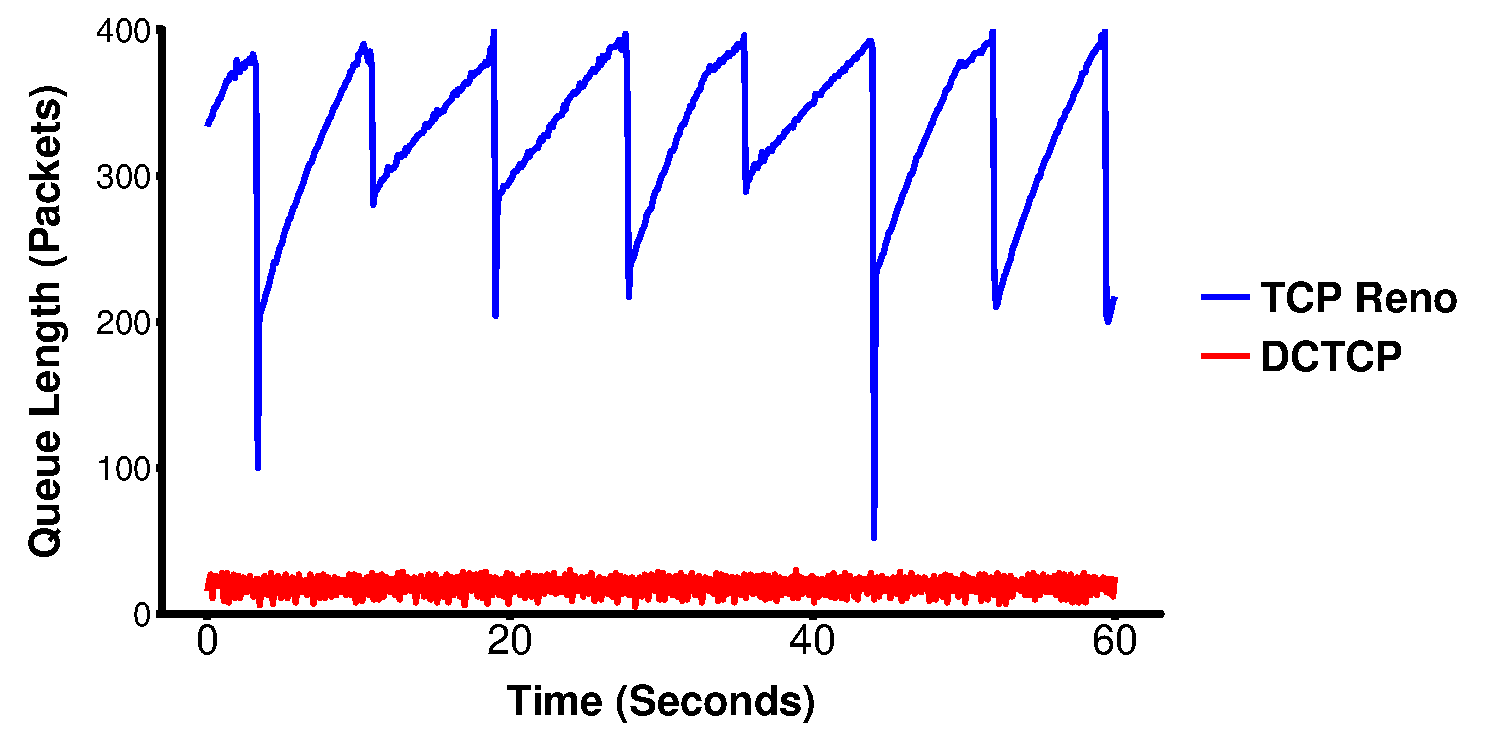
\includegraphics[height=1.75in,width=3.5in]{queue_2_flows}
\caption{Comparison of queue length over time between DCTCP and TCP Reno with 2 flows}
\end{figure}

\begin{figure}
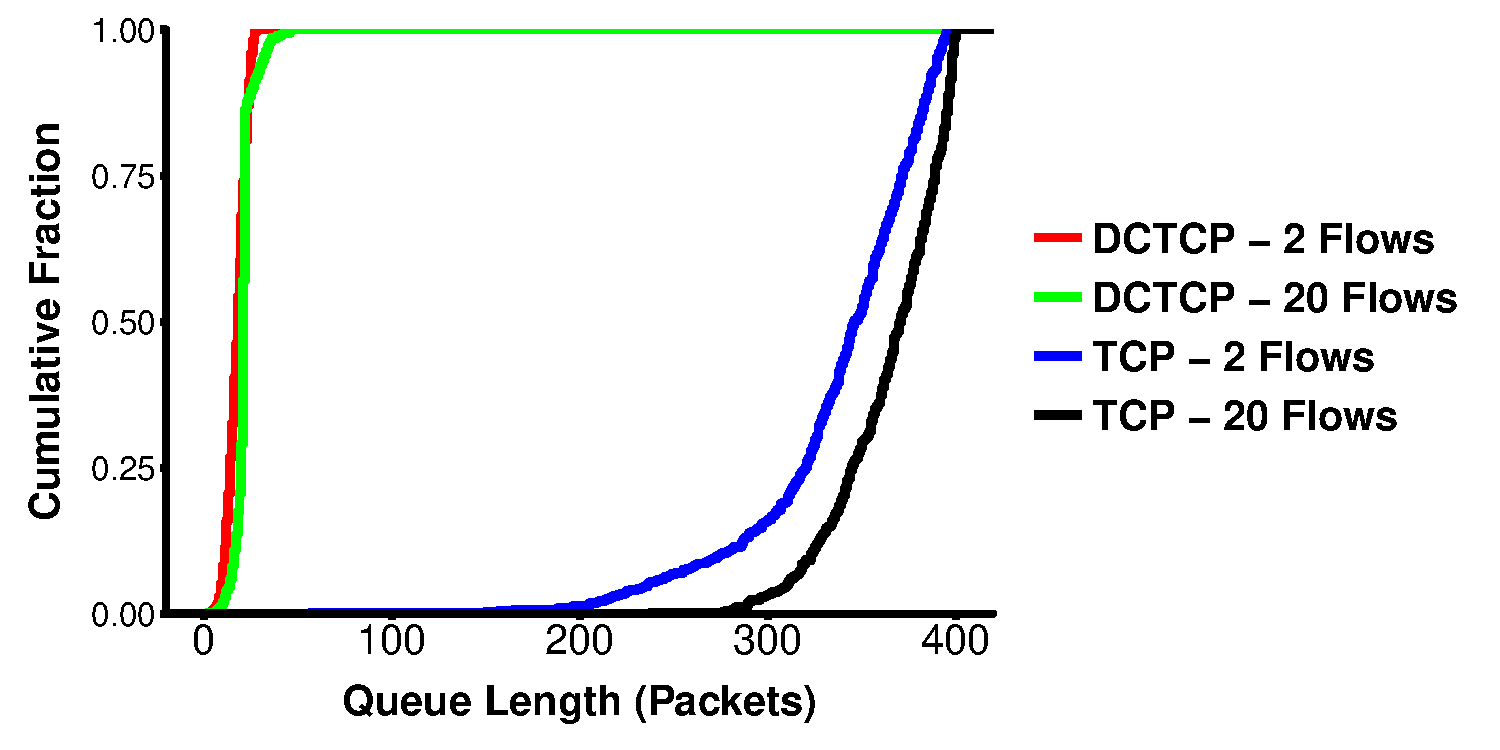
\includegraphics[height=1.75in,width=3.5in]{queue_cdf}
\caption{CDF of queue length for DCTCP and TCP Reno with 2 and 20 flows}
\end{figure}

\subsubsection{Throughput}

The model presented by the authors suggests setting $K$ as a function of both link speed and RTT, and showed that throughput was insensitive to low values of $K$ at link rates of 1Gbps. Since an initial attempt to reproduce these findings with an RTT of 100$\mu$s at a link rate of 100 Mbps confirmed that throughput is insensitive to $K$ when both RTT and link speeds are low, the RTT was increased to 10 ms to compensate for limited bandwidth and the test was repeated. Figure 3 shows the total throughput of two flows transferring data to a single receiver as a function of the marking threshold, $K$. The results under these conditions showed that throughput increased with $K$ until the maximum throughput was reached at $K \approx 12$.

The original authors suggest selecting $K > (C \times RTT) / 7$ where $K$ is the marking threshold, $C$ is the bottleneck capacity in packets/second, and $RTT$ is the round trip time in seconds. The network configuration used in this test used 1500 byte packets, meaning that the bottleneck could handle 8333 packets/second. Plugging in an RTT of 10 gives $C = 8333$ and $RTT = 0.01$, for a suggested $K$ of 11.9 which closely matches the observed results. Thus, the results presented here validate the authors' model for selecting $K$ in network configurations where bandwidth is low and RTT is high relative to what might be observed in a typical data center.

\begin{figure}
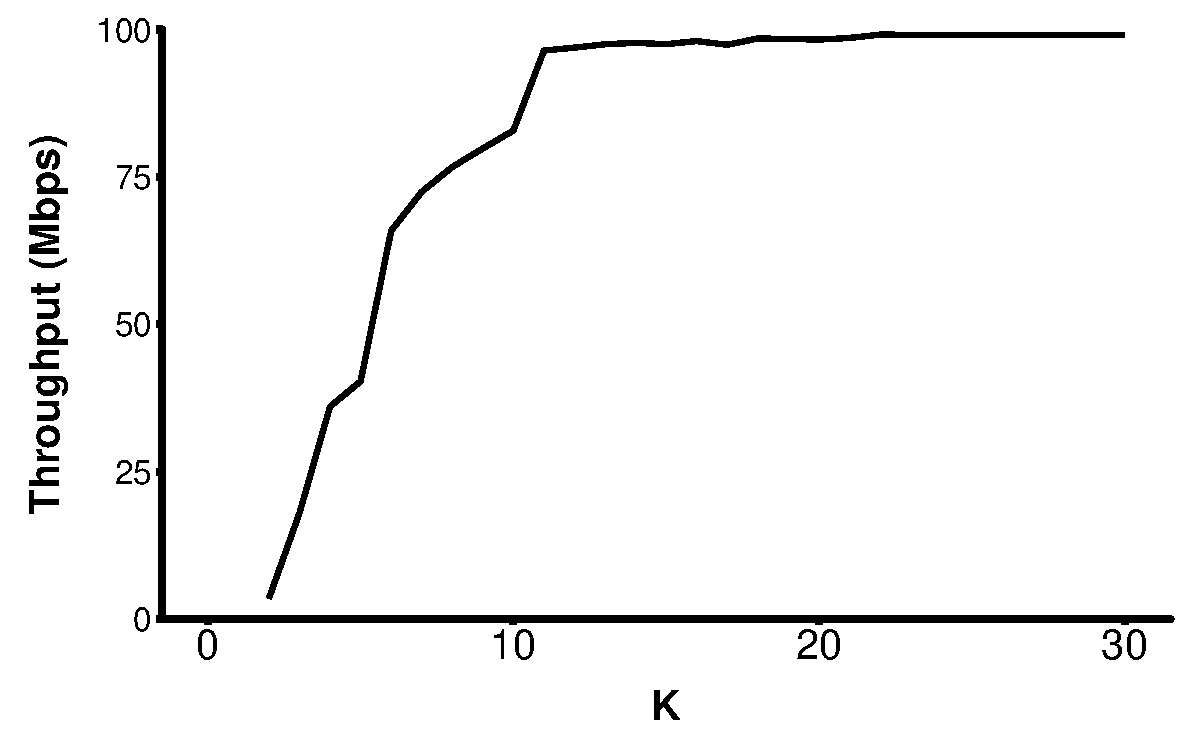
\includegraphics[height=1.75in,width=3in]{k_throughput_delay}
\caption{Throughput as a function of K}
\end{figure}

\subsubsection{Convergence}

Convergence was tested by incrementally starting 5 flows transmitting to a single receiver across a shared bottleneck and allowing each to run for 60 seconds before adding the next flow. Once the fifth flow had run for 60 seconds, each of the 5 flows was stopped in 60 second intervals in reverse of the order in which they were added. The results of the DCTCP convergence test (see Figure 4) show that each of the DCTCP flows converges to its fair share of the available bandwidth with little variability. In addition, the total bandwidth across all flows indicated consistently high throughput as flows were started and stopped, further confirming that DCTCP makes full use of available bandwidth.

Interestingly, the results of the TCP New Reno convergence test showed considerably more variability than the results of the DCTCP convergence test (see Figure 5). While the original authors noted that their TCP New Reno tests showed greater variability than DCTCP, the variability observed here is substatially more dramatic than in the original results. The cause of this greater perceived variability could be due to differences in network bandwidth, with TCP New Reno showing proportionally more variability in the lower bandwidth tests presented here, or could be a result of differences between the real hardware used in the original paper and the emulated Mininet topology used here.

In addition, Jain's fairness index was calculated for both DCTCP and TCP New Reno. As shown by the original authors, DCTCP had a fairness index of 0.99, indicating that DCTCP flows converge to their fair share of bandwidth utilization. Similarly, TCP New Reno had a fairness index of 0.99, indicating that New Reno acheived fairness between flows despite the observed variability in throughput. 

\begin{figure}
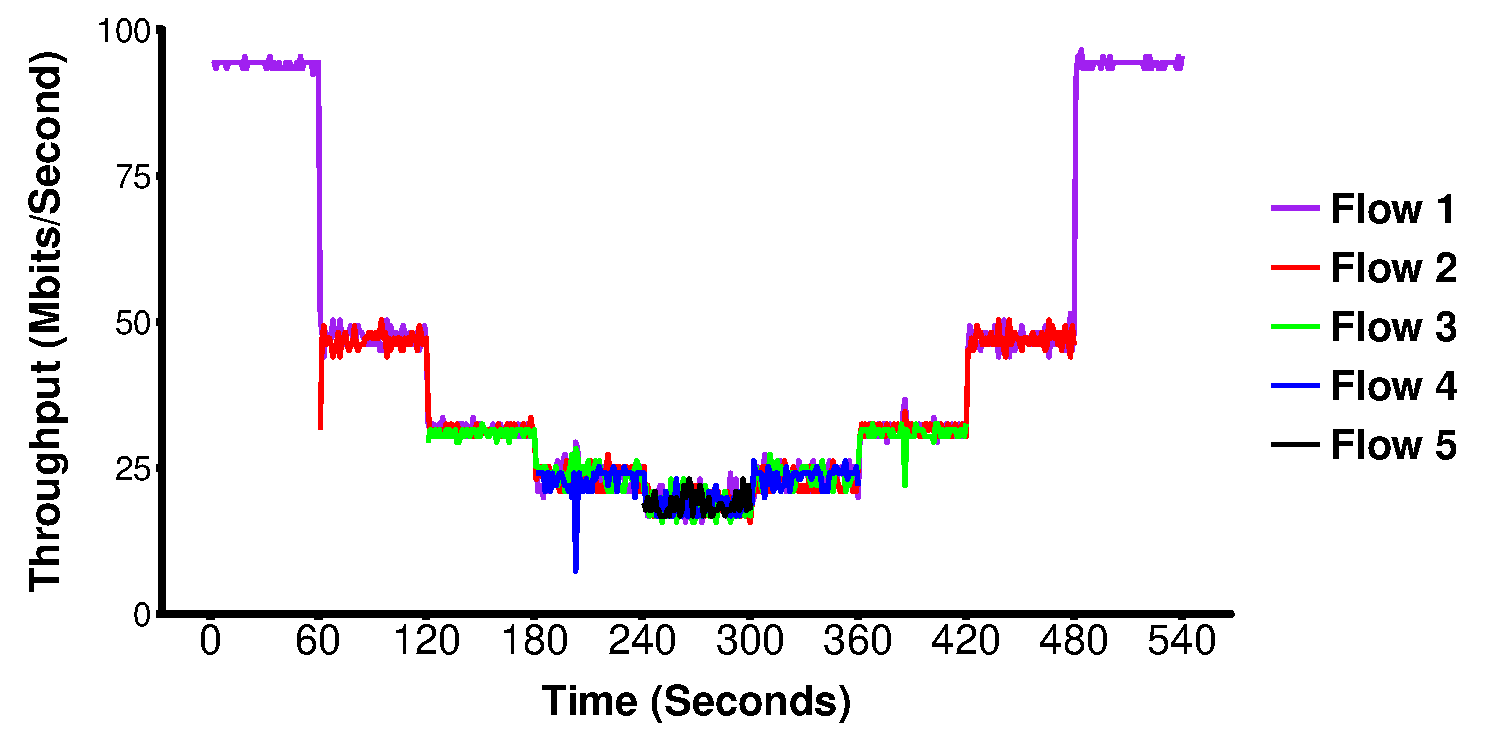
\includegraphics[height=1.75in,width=3.5in]{dctcp_converg}
\caption{Convergence of 5 flows DCTCP}
\end{figure}

\begin{figure}
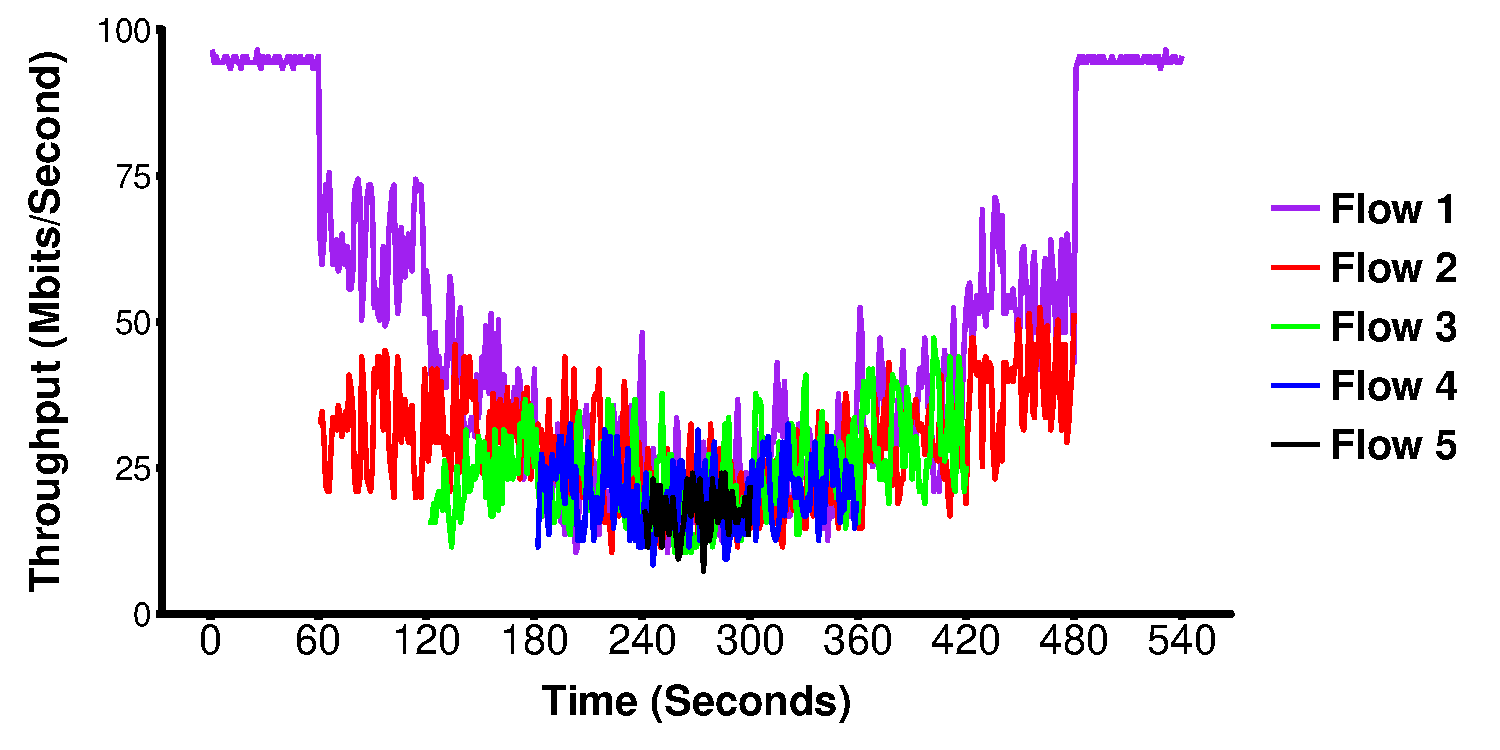
\includegraphics[height=1.75in,width=3.5in]{reno_converg}
\caption{Convergence of 5 flows TCP Reno}
\end{figure}

\subsection{Limitations}

The major limitation with this attempt to reproduce DCTCP performance tests is that Mininet could not reliably sustain speeds above 100 Mbps, making it difficult to relate the results presented here to conditions typical of real data centers.

\section{Conclusions}

